\documentclass[pre,twocolumn,superscriptaddress,nofootinbib]{revtex4-2}
\usepackage{amsmath,amssymb,bm,graphicx,xspace}
\usepackage[hidelinks]{hyperref}
\newcommand{\E}{\mathbb{E}}
\newcommand{\pOp}{p_{\mathrm{op}}}
\newtheorem{proposition}{Proposition}
\newtheorem{corollary}{Corollary}
\newtheorem{lemma}{Lemma}
% generated by reproducibility_pre/scripts/P1_numbers.py -- do not edit
\newcommand{\EpPca}{\ensuremath{0.035}\xspace}
\newcommand{\EpSurMed}{\ensuremath{0.0027}\xspace}
\newcommand{\EpSurQ}{\ensuremath{0.0070}\xspace}
\newcommand{\EpSurMax}{\ensuremath{0.0117}\xspace}
\newcommand{\NSur}{\ensuremath{200}\xspace}
\newcommand{\EpObsOverMax}{\ensuremath{3.0}\xspace}
\newcommand{\EpWinObs}{\ensuremath{0.15}\xspace}
\newcommand{\EpWinSurMed}{\ensuremath{0.13}\xspace}
\newcommand{\OmFitSqRatio}{\ensuremath{8.5}\xspace}
\newcommand{\GRatio}{\ensuremath{1.5}\xspace}
\newcommand{\GPca}{\ensuremath{47}\xspace}
\newcommand{\OmFitPca}{\ensuremath{0.019}\xspace}
\newcommand{\EpRevRefit}{\ensuremath{0.095}\xspace}
\newcommand{\OmFitRevRefit}{\ensuremath{0.034}\xspace}
\newcommand{\GRevRefit}{\ensuremath{41}\xspace}
\newcommand{\EpRevFixed}{\ensuremath{0.038}\xspace}
\newcommand{\OmFitRevFixed}{\ensuremath{0.020}\xspace}
\newcommand{\OmWinFwd}{\ensuremath{-0.020}\xspace}
\newcommand{\OmWinRev}{\ensuremath{-0.020}\xspace}
\newcommand{\OmLevFwd}{\ensuremath{+0.028}\xspace}
\newcommand{\OmLevRev}{\ensuremath{-0.028}\xspace}
\newcommand{\OmLevCen}{\ensuremath{+0.027}\xspace}
\newcommand{\OmLevData}{\ensuremath{+0.0276}\xspace}
\newcommand{\DDO}{\ensuremath{+0.0057}\xspace}
\newcommand{\DDP}{\ensuremath{+0.0165}\xspace}
\newcommand{\DDCen}{\ensuremath{-0.0018}\xspace}
\newcommand{\OmPcaFwd}{\ensuremath{+0.020}\xspace}
\newcommand{\OmPcaRev}{\ensuremath{-0.021}\xspace}
\newcommand{\OmPcaCen}{\ensuremath{+0.016}\xspace}
\newcommand{\OPcaRev}{\ensuremath{-0.0004}\xspace}
\newcommand{\OPcaCen}{\ensuremath{+0.0035}\xspace}
\newcommand{\CryptoPmax}{\ensuremath{0.003}\xspace}
\newcommand{\SELevP}{\ensuremath{0.0021}\xspace}
\newcommand{\LevPz}{\ensuremath{13}\xspace}
\newcommand{\PcaPz}{\ensuremath{11}\xspace}
\newcommand{\WinOz}{\ensuremath{12}\xspace}
\newcommand{\SERatioLo}{\ensuremath{0.5}\xspace}
\newcommand{\SERatioHi}{\ensuremath{1.4}\xspace}
\newcommand{\CryptoLevPz}{\ensuremath{0.9}\xspace}
\newcommand{\DDLoadOne}{\ensuremath{-0.50}\xspace}
\newcommand{\DDLoadTwo}{\ensuremath{-0.27}\xspace}
\newcommand{\VolMaxDiff}{\ensuremath{1.4\times10^{-5}}\xspace}
\newcommand{\VolAdj}{\ensuremath{4.152\times10^{9}}\xspace}
\newcommand{\OmTabOne}{\ensuremath{-0.0135}\xspace}
\newcommand{\OmFitTabOne}{\ensuremath{-0.0127}\xspace}
\newcommand{\GTabOne}{\ensuremath{1.5\times10^{4}}\xspace}
\newcommand{\EpTabOne}{\ensuremath{4.8}\xspace}
\newcommand{\EpNoiseOne}{\ensuremath{0.21}\xspace}
\newcommand{\EpNoiseTen}{\ensuremath{0.015}\xspace}
\newcommand{\OmNoiseOne}{\ensuremath{1\%}\xspace}
\newcommand{\OmNoiseTen}{\ensuremath{9\%}\xspace}
\newcommand{\OmFitDevLo}{\ensuremath{3}\xspace}
\newcommand{\OmFitDevHi}{\ensuremath{11}\xspace}
\newcommand{\EllTabOne}{\ensuremath{0.10}\xspace}
\newcommand{\SimMaxErr}{\ensuremath{3.3\%}\xspace}
\newcommand{\MCDevMax}{\ensuremath{1.5\%}\xspace}
\newcommand{\MCDevNineNine}{\ensuremath{9\%}\xspace}
\newcommand{\SingleErrLo}{\ensuremath{+0.14}\xspace}
\newcommand{\SingleErrHi}{\ensuremath{+0.50}\xspace}
\newcommand{\TwoErrLo}{\ensuremath{-0.14}\xspace}
\newcommand{\TwoErrHi}{\ensuremath{+0.03}\xspace}
\newcommand{\TwoErrAbs}{\ensuremath{0.14}\xspace}
\newcommand{\SingleFacLo}{\ensuremath{1.7}\xspace}
\newcommand{\SingleFacHi}{\ensuremath{4.1}\xspace}
\newcommand{\ClfEst}{\ensuremath{0.84}\xspace}
\newcommand{\ClfExact}{\ensuremath{0.53}\xspace}
\newcommand{\DWEpOne}{\ensuremath{7.7}\xspace}
\newcommand{\DWEpEighty}{\ensuremath{1.5}\xspace}
\newcommand{\DWLatLo}{\ensuremath{2.9}\xspace}
\newcommand{\DWLatHi}{\ensuremath{3.7}\xspace}
\newcommand{\DWPredOne}{\ensuremath{7.1}\xspace}
\newcommand{\SVQnfMax}{\ensuremath{0.009}\xspace}
\newcommand{\SVMatchLo}{\ensuremath{0.022}\xspace}
\newcommand{\SVMatchHi}{\ensuremath{0.047}\xspace}
\newcommand{\TOneLevMax}{\ensuremath{+0.027}\xspace}
\newcommand{\TOneEpAtMax}{\ensuremath{0.032}\xspace}
\newcommand{\RRobs}{\ensuremath{+1.03}\xspace}
\newcommand{\RRlo}{\ensuremath{-0.71}\xspace}
\newcommand{\RRhi}{\ensuremath{0.84}\xspace}
\newcommand{\RRp}{\ensuremath{0.01}\xspace}
\newcommand{\LamMkt}{\ensuremath{0.020}\xspace}
\newcommand{\EllMktPair}{\ensuremath{0.10}\xspace}
\newcommand{\EllWinFive}{\ensuremath{0.11}\xspace}
\newcommand{\EllWinTwenty}{\ensuremath{0.40}\xspace}
\newcommand{\EllWinSixty}{\ensuremath{0.72}\xspace}
\newcommand{\EllWinTwoFifty}{\ensuremath{0.95}\xspace}
\newcommand{\EllMktRV}{\ensuremath{0.45}\xspace}
\newcommand{\EllMktPca}{\ensuremath{0.49}\xspace}
\newcommand{\EllCheckDiff}{\ensuremath{0.003}\xspace}
% result numbers, written by reproducibility_pre/scripts/P1_numbers.py
\InputIfFileExists{supp_labels}{}{}% supplemental table numbers, written by sync_labels.py
\newcommand{\Sref}[1]{\ifcsname supp@#1\endcsname\csname supp@#1\endcsname\else S??\fi}
% ---- submission metadata: filled at release; see ZENODO_DEPOSIT.md in the repository root
\newcommand{\ZenodoDOI}{\textbf{[DOI of the new Zenodo version]}}% fill after the Zenodo v2.0.0 deposit
\newcommand{\RepoCommit}{\textbf{[commit hash]}}% fill with the release commit
\newenvironment{proof}{\par\noindent\emph{Proof.}\ }{\hfill$\square$\par}
\makeatletter\g@addto@macro\UrlBreaks{\do\_\do\/\do\.\do-}\makeatother
\renewcommand{\dbltopfraction}{0.92}\renewcommand{\topfraction}{0.92}\renewcommand{\textfraction}{0.06}
\renewcommand{\floatpagefraction}{0.85}\renewcommand{\dblfloatpagefraction}{0.85}

\begin{document}

\title{Observer-induced irreversibility in trailing-window early-warning states}

\author{Boyan Xing}
\email{t330025089@mail.bnbu.edu.cn}
\affiliation{Department of Mathematical Sciences, Faculty of Science and Technology, Beijing Normal-Hong Kong Baptist University, Zhuhai, Guangdong, China}
\author{Jiayi Pan}
\affiliation{Department of Accounting, Faculty of Business and Management, Beijing Normal-Hong Kong Baptist University, Zhuhai, Guangdong, China}

\date{\today}

\begin{abstract}
Early-warning indicators are built from trailing windows. For linear filters of a stationary multichannel input, the lag-one antisymmetry---the discrete area-enclosing rate that sets the current of a fitted linear Markov model---splits exactly into an observer term, which needs windows with different centers, and a physical term, which needs time-antisymmetric input covariances; time reversal of the data separates the two without a model. Windows of a single signal therefore show only observer-made irreversibility at second order, and the entropy production of a fitted two-dimensional model factorizes into the squared antisymmetry and an innovation-geometry factor that makes reversible inputs look strongly dissipative. The same windows destroy transition information, in closed form for Gaussian inputs. In daily S\&P 500 data the volatility windows carry an observer term as large as in time-reversible surrogates, and the physical term is the leverage effect.
\end{abstract}

\maketitle

\section{Introduction}\label{sec:intro}

A linear Markov model fitted to the 5- and 20-day realized volatility of the S\&P 500 reports an entropy production of \EpWinObs per day. Fitted to surrogate data whose volatility is time reversible by construction, the same model reports \EpWinSurMed. Most of what the fitted model calls dissipation is made by the way the state was observed: two trailing averages of one signal, the shorter of which systematically leads the longer. Trailing windows of this kind are the standard preprocessing of early-warning indicators for critical transitions \cite{scheffer2009,kuehn2011,dakos2012,lenton2012}, and the currents fitted to windowed states are not idle: time irreversibility, measured by the difference between forward and backward cross-correlations, has been proposed as an early-warning signal \cite{kooloth2026,xu2023}, and forecasts of the committor type integrate a drift fitted to such a state \cite{xing2026b}; both inherit whatever the observer adds. The fitted model is misspecified---a windowed state is not Markov---but its drift and current are what such pipelines compute, so its irreversibility is the quantity to account for. We ask what trailing windows do to a stochastic transition, and how much of the irreversibility of a windowed state belongs to the system.

Two effects are at stake. Windows compress the state and destroy transition information that the latent process still carries, which limits what any early-warning statistic can detect and how skillful it can be \cite{boettiger2012,ditlevsen2010,duplessis2026}. And a coarse-graining that does not commute with time reversal can create apparent irreversibility, whereas one that commutes bounds the true entropy production from below \cite{martinez2019,hartich2024,bisker2024,esposito2012}; conversely, scalar observation of a linear system can hide its currents \cite{lucente2022prr}. Trailing windows do not commute with time reversal. The same construction is the belief rule of extrapolative investors in behavioral finance \cite{bgjs2015}, an analogy we use only for orientation.

Our results are four. (i) For linear filters of any stationary multichannel input, the lag-one antisymmetry---the discrete-time area-enclosing rate, which sets the current of a fitted linear Markov model---splits exactly into an observer term and a physical term, and time reversal of the data separates them without a model (Sec.~\ref{sec:theory}, Proposition~\ref{prop:decomp}). (ii) The entropy production of a fitted two-dimensional model factorizes into the squared antisymmetry and an innovation-geometry factor, which explains why reversible inputs can look strongly dissipative (Proposition~\ref{prop:factor}). (iii) The information lost to compression is a closed-form series for an Ornstein--Uhlenbeck input (Lemma~\ref{lem:mehler}) and is governed by two rates, local curvature and Kramers switching, in a double well (Sec.~\ref{sec:info}). (iv) In daily S\&P 500 data, time reversal, centered windows and sign randomization identify the observer term in the volatility windows and the leverage effect as the physical term; a stochastic-volatility model with leverage accounts for both, and the same model shows that the market's windows lose about half of the information that the latent volatility carries about its next excursion (Sec.~\ref{sec:market}).

Time-series irreversibility is measured by symbolic statistics \cite{daw2000}, by asymmetry indices of physiological series \cite{porta2008}, by visibility graphs \cite{lacasa2012}, also applied to financial series \cite{flanagan2016}, and by many other estimators \cite{zanin2021}; for linear processes reversibility criteria are classical \cite{weiss1975,tong2005,chan2006}, and the antisymmetric part of lagged cross-correlations is an established nonequilibrium measure, as the stochastic area or area-enclosing rate of linear systems \cite{ghanta2017,gonzalez2019} and as the cycling frequency of probability-flux analysis \cite{gradziuk2019,battle2016}. When only part of a system is observed, entropy production is bounded or inferred from coarse-grained trajectories \cite{roldan2010,roldan2012}, from waiting times and visible transitions \cite{skinner2021,harunari2022,vandermeer2022}, and exactly for coarse-grainings that preserve it \cite{teza2020}. These works ask how hidden degrees of freedom or projections change the measured irreversibility. Here the observable is a causal filter of the signal, and the question is how much irreversibility the temporal offsets of its kernels add.

In finance, time-reversal asymmetry of returns is a known stylized fact, traced to multi-timescale volatility feedback \cite{zumbach2009,lynch2003,chicheportiche2014} and to the leverage effect \cite{black1976,bouchaud2001}. What is new here is the exact split of the area-enclosing rate of causally filtered observables into an observer part, set by the kernel offsets, and a physical part, together with a model-free estimator from time-reversed data [Eq.~\eqref{eq:estimator}], its consequences for windowed indicators, and the measurement of both parts in an early-warning pipeline applied to market data. The split also shows which kind of financial time asymmetry a second-order trailing-window state can see: the leverage asymmetry between channels, not the higher-order asymmetry of volatility itself.

\section{Observer-induced irreversibility of filtered signals}\label{sec:theory}

\subsection{Setting and the time-reversal decomposition}\label{sec:decomp}

Any linear filter of a stationary multichannel signal produces a lag-one antisymmetry that splits exactly into an observer term and a physical term. Let $u_t=(u^1_t,\dots,u^P_t)$ be a jointly stationary input with cross-covariances
\begin{equation}
\gamma_{pq}(\tau)=\mathrm{Cov}(u^p_{t+\tau},u^q_t),\qquad \gamma_{qp}(\tau)=\gamma_{pq}(-\tau),
\end{equation}
and let an observer form the state $y(t)=(y_1,\dots,y_m)$ from causal filters,
\begin{equation}
y_i(t)=\sum_{a\ge0}k_i(a)\,u^{p_i}_{t-a},
\end{equation}
where $p_i$ labels the input channel of observable $i$; a trailing mean of width $w_i$ has $k_i(a)=1/w_i$ for $0\le a<w_i$. With $C(s)=\mathrm{Cov}[y(t+s),y(t)]$, time reversibility of a stationary process requires $C(s)=C(s)^\top$ for all $s$; for a Gaussian process the condition is also sufficient, because second moments fix its law, and reversibility criteria for linear non-Gaussian processes are classical \cite{weiss1975,tong2005,chan2006}. The leading time-reversal-odd statistic is the standardized lag-one antisymmetry
\begin{equation}
\omega_{ij}=\frac{C_{ij}(1)-C_{ji}(1)}{2\sqrt{C_{ii}(0)C_{jj}(0)}} .\label{eq:omega}
\end{equation}
In standardized coordinates $\omega_{ij}$ is minus the mean signed area swept per step by the trajectory in the $(y_i,y_j)$ plane, i.e.\ the discrete-time area-enclosing rate \cite{ghanta2017,gonzalez2019}, closely related to the cycling frequencies of probability-flux analysis \cite{gradziuk2019,battle2016}; for the linear Markov model fitted to $y$ it sets the stationary current (Sec.~\ref{sec:factor}). Define the cross-correlation of two kernels,
\begin{equation}
K_{ij}(m)=\sum_a k_i(a)\,k_j(a+m),\qquad K_{ji}(m)=K_{ij}(-m),
\end{equation}
and write $f^\pm$ for the even and odd parts of a sequence, $f^\pm(m)=\tfrac12[f(m)\pm f(-m)]$. For a covariance sequence $\gamma$ we write $\Delta\gamma^\pm\equiv\Delta(\gamma^\pm)$ for the difference operator applied to its even and odd parts, $(\Delta\gamma^\pm)(m)=\gamma^\pm(m+1)-\gamma^\pm(m-1)$; $\Delta\gamma^+$ is odd and $\Delta\gamma^-$ is even.

\begin{proposition}[Time-reversal decomposition]\label{prop:decomp}
With $\gamma\equiv\gamma_{p_ip_j}$ and $\Delta\gamma(m)=\gamma(m+1)-\gamma(m-1)$,
\begin{equation}
C_{ij}(1)-C_{ji}(1)=\sum_m K_{ij}(m)\,\Delta\gamma(m).\label{eq:decomp}
\end{equation}
Consequently $\omega_{ij}=O_{ij}+P_{ij}$ with
\begin{align}
O_{ij}&=\frac{1}{2\sigma_i\sigma_j}\sum_m K^-_{ij}(m)\,\Delta\gamma^+(m),\label{eq:O}\\
P_{ij}&=\frac{1}{2\sigma_i\sigma_j}\sum_m K^+_{ij}(m)\,\Delta\gamma^-(m),\label{eq:P}
\end{align}
$\sigma_i^2=C_{ii}(0)$. Under time reversal of the input, $O_{ij}\to O_{ij}$ and $P_{ij}\to-P_{ij}$.
\end{proposition}

\begin{proof}
Substituting $b=a+m$ in $C_{ij}(s)=\sum_{a,b}k_i(a)k_j(b)\,\gamma(s-a+b)$ gives $C_{ij}(s)=\sum_mK_{ij}(m)\gamma(s+m)$. With $K_{ji}(m)=K_{ij}(-m)$ and $\gamma_{p_jp_i}(\tau)=\gamma(-\tau)$, $C_{ji}(1)=\sum_mK_{ij}(m)\gamma(m-1)$, which is Eq.~\eqref{eq:decomp}. Write $K_{ij}=K^+_{ij}+K^-_{ij}$ and $\Delta\gamma=\Delta\gamma^++\Delta\gamma^-$. The difference operator maps even sequences to odd ones and odd sequences to even ones, so the products $K^+_{ij}\Delta\gamma^+$ and $K^-_{ij}\Delta\gamma^-$ are odd in $m$ and sum to zero. The surviving products, $K^-_{ij}\Delta\gamma^+$ (odd times odd) and $K^+_{ij}\Delta\gamma^-$ (even times even), are even and give Eqs.~\eqref{eq:O} and \eqref{eq:P}. Time reversal maps $\gamma_{pq}(\tau)\to\gamma_{pq}(-\tau)$, hence $\gamma^+\to\gamma^+$ and $\gamma^-\to-\gamma^-$, and leaves $\sigma_i^2=\sum_mK_{ii}(m)\gamma^+_{p_ip_i}(m)$ unchanged.
\end{proof}

The observer term needs kernels whose cross-correlation is not symmetric, i.e.\ windows with different temporal centers; it is built from the time-symmetric part of the input covariances. The physical term needs an odd cross-covariance between input channels, i.e.\ genuine time asymmetry of the input. Proposition~\ref{prop:decomp} yields a model-free estimator: rebuilding the features from the time-reversed input gives $\omega^{\rm rev}_{ij}=O_{ij}-P_{ij}$, so
\begin{equation}
O_{ij}=\tfrac12(\omega_{ij}+\omega^{\rm rev}_{ij}),\qquad P_{ij}=\tfrac12(\omega_{ij}-\omega^{\rm rev}_{ij}).\label{eq:estimator}
\end{equation}
For nonlinear features (logarithms, running maxima) the decomposition holds to linear order. Equation~\eqref{eq:estimator} nevertheless remains an exact split of any statistic into its time-reversal-even and time-reversal-odd parts, and Sec.~\ref{sec:market} measures how close this split is to the linear one.

\begin{figure*}[t]
\centering
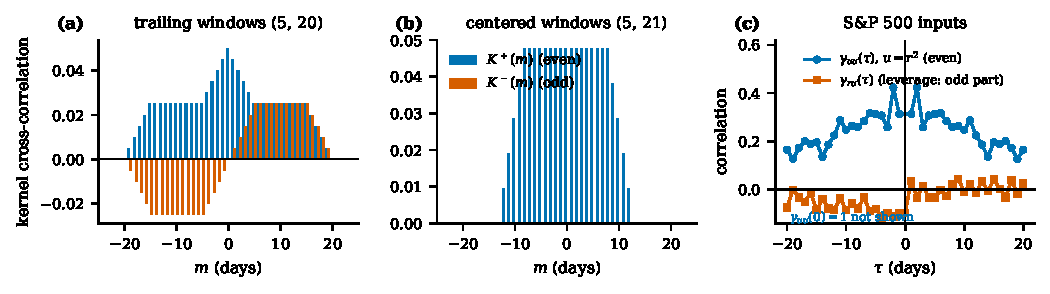
\includegraphics[width=\textwidth]{figures/fig1_decomposition.pdf}
\caption{The two ingredients of Proposition~\ref{prop:decomp}. (a) Trailing windows of 5 and 20 days: the cross-correlation $K(m)$ of the two kernels has an odd part, because the window centers differ by 7.5 days. (b) Centered windows of 5 and 21 days: $K^-\equiv0$, so no observer term arises. (c) Inputs from the S\&P 500: the autocorrelation of squared returns is even, whereas the cross-correlation $\mathrm{Corr}(r_{t+\tau},r_t^2)$ is negative for $\tau<0$ and near zero for $\tau>0$---returns precede volatility, and this odd part is the leverage effect.}
\label{fig:decomp}
\end{figure*}

\subsection{Two corollaries}\label{sec:corollaries}

Windows of one scalar signal are blind, at second order, to the irreversibility of that signal.

\begin{corollary}[Single-channel blindness]\label{cor:single}
If all observables filter the same scalar input, then $P_{ij}\equiv0$, and $C(0)$ and $C(1)$ are identical for the input and its time reversal. Every quantity computed from $C(0)$ and $C(1)$---the antisymmetry, the drift, current and entropy production of the fitted linear Markov model, and the Gaussian Markov Kullback--Leibler divergence---is therefore the same for a process and its time reversal.
\end{corollary}

\begin{corollary}[Symmetric kernels]\label{cor:symmetric}
If all kernels are symmetric about a common center (centered windows of any widths), or all kernels are equal (equal-width trailing windows), then $K_{ij}$ is even and $O_{ij}\equiv0$.
\end{corollary}

Corollary~\ref{cor:single} restates the elementary fact that the second-order statistics of a scalar stationary process are time symmetric; its content here is that every quantity a linear early-warning pipeline computes from windows of one signal inherits this symmetry, so any current such a pipeline reports is made by the observer. It is the second-order face of a general fact: a coarse-graining that does not commute with time reversal can create apparent irreversibility, whereas a commuting one bounds the true entropy production from below \cite{martinez2019,hartich2024,bisker2024,esposito2012}; Corollary~\ref{cor:symmetric} identifies the commuting linear filters. The classical observation that moving averages of random series generate spurious oscillations \cite{slutzky1937} concerns a single filtered series and is time symmetric; the effect here needs two kernels with different temporal centers. Conversely, scalar observation can hide the currents of a linear system \cite{lucente2022prr}.

\subsection{Entropy production of the fitted model}\label{sec:factor}

The entropy production of a fitted two-dimensional linear model is the squared antisymmetry times a factor set by the geometry of its innovations. Least squares of $y_{t+1}-y_t$ on $y_t$ gives, in the population, $\Phi=C(1)C(0)^{-1}$, the drift per step $A=\Phi-I$ and the residual covariance $D=C(0)-\Phi C(0)\Phi^\top$. Read as the Ornstein--Uhlenbeck (OU) process $dZ=AZ\,dt+G\,dW$ with $GG^\top=D$ and stationary covariance $\Sigma$ ($A\Sigma+\Sigma A^\top+D=0$), the fitted model carries the current $J(z)=\Omega\Sigma^{-1}z\,\rho(z)$, $\Omega=\tfrac12(A\Sigma-\Sigma A^\top)$, and the entropy production per step \cite{seifert2012}
\begin{equation}
\dot e_p=2\,\mathrm{tr}\big(\Sigma^{-1}\Omega^\top D^{-1}\Omega\big).\label{eq:ep}
\end{equation}
In two dimensions $\Omega=\omega_{\rm fit}\,\mathsf J$ with $\mathsf J=\bigl(\begin{smallmatrix}0&1\\-1&0\end{smallmatrix}\bigr)$, and $\mathsf J^\top D^{-1}\mathsf J=D/\det D$.

\begin{proposition}[Factorization]\label{prop:factor}
For a fitted two-dimensional OU model,
\begin{equation}
\dot e_p=2\,\omega_{\rm fit}^2\,\mathcal G,\qquad
\mathcal G=\frac{\mathrm{tr}(\Sigma^{-1}D)}{\det D}=\frac{1}{d_{\min}}+\frac{1}{d_{\max}},\label{eq:factor}
\end{equation}
where $d_{\min}\le d_{\max}$ are the eigenvalues of $D$ in coordinates whitened by $\Sigma$.
\end{proposition}

In standardized coordinates $\omega_{\rm fit}$ differs from the antisymmetry~\eqref{eq:omega} only through $\Sigma\neq C(0)$ (by \OmFitDevLo--\OmFitDevHi\% for the Gaussian observer below). The geometry factor $\mathcal G$ diverges when the innovations of the two observables are nearly collinear, which is exactly what happens for two windows of one signal: both are driven by the same newest input value. The size of $\dot e_p$ then reports innovation geometry rather than the strength of the current.

\subsection{Gaussian observer}\label{sec:gauss}

For a unit OU input $dx=-\lambda x\,dt+\sqrt{2\lambda}\,dW$ sampled at unit spacing [an AR(1) with $\phi=e^{-\lambda}$] and observed through trailing means of widths $(w,4w)$, every quantity is in closed form (Appendix~\ref{app:gauss}); by Corollary~\ref{cor:single}, $\omega=O$. Table~\ref{tab:gauss} lists them at $\phi=0.98$. At $\lambda w=0.1$ the antisymmetry is only \OmTabOne ($\omega_{\rm fit}=\,$\OmFitTabOne in the fitted model), yet the fitted model reports an entropy production of \EpTabOne per step for a process with none: $2\omega_{\rm fit}^2\mathcal G=\,$\EpTabOne because $\mathcal G=\,$\GTabOne. The current has the direction of the lag: an excursion of the input moves the short window first and the long one later, so the trajectory circulates counterclockwise in the $(y_1,y_2)$ plane and $\omega<0$ in every row of Table~\ref{tab:gauss}. Independent white observation noise of 1\% of the window variance changes $\omega$ by \OmNoiseOne but lowers $\dot e_p$ to \EpNoiseOne; noise of 10\% lowers $\dot e_p$ to \EpNoiseTen, while $\omega$ changes by \OmNoiseTen, only through the noise-inflated variances [Fig.~\ref{fig:gauss}(b,c)]. Centered windows give zero to sampling accuracy (Corollary~\ref{cor:symmetric}), and $3\times10^5$-step simulations reproduce the closed forms of the flux-to-drift ratio, $\dot e_p$ and the Gaussian Markov Kullback--Leibler divergence $d_1$ within \SimMaxErr (Supplemental Material \cite{SM}, Table~\Sref{gauss}). Because all observables are filters of one scalar signal, the spectral matrix of $y$ has rank one and the forward and backward path measures are mutually singular, so the full-path divergence is infinite; Eq.~\eqref{eq:factor} shows how this singularity enters the fitted model through $d_{\min}\to0$.

A metastable input behaves in the same way. For the double well of Sec.~\ref{sec:dw} with $\tau_c=\infty$, seen through two trailing windows $(w,4w)$ of $x$ alone, the input is scalar and reversible, so by Corollary~\ref{cor:single} any fitted current is made by the observer; the fitted OU model nevertheless reports $\dot e_p=\,$\DWEpOne per step at $w=1$, falling to \DWEpEighty at $w=80$ [Fig.~\ref{fig:dw}(c)]. For finite $\tau_c$ the latent $(x,c)$ process carries a genuine current, but only (\DWLatLo--\DWLatHi)$\times10^{-3}$ per step by the same estimator (Table~\Sref{dwcurrent}), three orders of magnitude less, and Proposition~\ref{prop:factor} attributes the excess to nearly collinear innovations. The Gaussian observer with the local stiffness $\bar\lambda$ predicts the short-window value (\DWPredOne at $w=1$) and falls below it at wide windows, where the slow hopping component dominates (Sec.~\ref{sec:dw}).

\begin{table*}[t]
\squeezetable
\caption{Gaussian observer, $\phi=0.98$, windows $(w,4w)$ in standardized coordinates: posterior variance $s^2$ of the latent state, lag-one antisymmetry $\omega$ [Eq.~\eqref{eq:omega}] and its fitted-model counterpart $\omega_{\rm fit}$, geometry factor $\mathcal G$ and entropy production $\dot e_p=2\omega_{\rm fit}^2\mathcal G$ (per step) of the fitted OU model, the same with observation noise $\eta^2=10^{-2}$ ($\dot e_p^{\,\eta}$), and the normalized information loss $\ell$ of a $2\sigma$ threshold forecast at a horizon of ten steps, as in Fig.~\ref{fig:gauss}(a).}
\label{tab:gauss}
\begin{ruledtabular}
\begin{tabular}{rcccccrrc}
$\lambda w$ & windows & $s^2$ & $\omega$ & $\omega_{\rm fit}$ & $\mathcal G$ & $\dot e_p$ & $\dot e_p^{\,\eta}$ & $\ell$\\
\hline
0.1 & (5,20) & 0.044 & $-$0.0135 & $-$0.0127 & $1.50\times10^{4}$ & 4.85 & 0.210 & 0.102\\
0.2 & (10,40) & 0.101 & $-$0.0121 & $-$0.0110 & $1.64\times10^{4}$ & 3.96 & 0.105 & 0.216\\
0.4 & (20,80) & 0.205 & $-$0.0098 & $-$0.0087 & $1.91\times10^{4}$ & 2.88 & 0.045 & 0.384\\
1.0 & (49,196) & 0.435 & $-$0.0058 & $-$0.0052 & $2.71\times10^{4}$ & 1.48 & 0.011 & 0.654\\
2.0 & (99,396) & 0.660 & $-$0.0031 & $-$0.0029 & $4.26\times10^{4}$ & 0.71 & 0.003 & 0.835\\
4.0 & (198,792) & 0.836 & $-$0.0015 & $-$0.0014 & $7.54\times10^{4}$ & 0.31 & 0.001 & 0.934\\
\end{tabular}
\end{ruledtabular}

\end{table*}

\section{Information loss}\label{sec:info}

Windows also destroy transition information, which we measure by the compression term of the Brier score. Let $Z$ be the latent Markov state, $E\in\{0,1\}$ an event, $\pOp(Z)=\mathrm P(E=1\mid Z)$ the oracle, $Y$ the observed state and $r^*(Y)=\mathrm P(E=1\mid Y)$. For any forecast $g(Y)$, orthogonality of the three differences gives the standard decomposition \cite{murphy1973,degroot1983,brocker2009}
\begin{align}
\E[(g-E)^2]&=\E[(g-r^*)^2]+\E[(r^*-\pOp)^2]\nonumber\\
&\quad+\E[\pOp(1-\pOp)]
\end{align}
into an estimation, a compression and a state-information term. The compression term, $L=\E[\mathrm{Var}(\pOp\mid Y)]$, is what the observer loses by seeing $Y$ instead of $Z$, whatever estimator it uses; we report it normalized, $\ell=L/\mathrm{Var}\,\pOp\in[0,1]$.

\subsection{Gaussian observer: an exact series}\label{sec:mehler}

For a reversible Ornstein--Uhlenbeck input the compression term is an exact Hermite series in the posterior variance. Given the windows $y_t$, the latent state is Gaussian with a mean linear in $y_t$ and a variance $s^2=1-c^\top C(0)^{-1}c$, $c_i=\mathrm{Cov}(x_t,y_i(t))$, that does not depend on the observed values.

\begin{lemma}[Mehler series]\label{lem:mehler}
If $\pOp$ has the normalized Hermite coefficients $a_n=\E[\pOp(X)\,\mathrm{He}_n(X)]/\sqrt{n!}$ under $X\sim N(0,1)$, then
\begin{equation}
L(s^2)=\sum_{n\ge1}a_n^2\big[1-(1-s^2)^n\big].\label{eq:mehler}
\end{equation}
$L$ increases from $L(0)=0$ to $L(1)=\mathrm{Var}\,\pOp$, and $L'(0)=\E[\pOp'(X)^2]\ge\mathrm{Var}\,\pOp$.
\end{lemma}

This is the classical Hermite (Mehler) expansion of the Ornstein--Uhlenbeck semigroup \cite{mehler1866,odonnell2014}, applied to the posterior of the latent state (Appendix~\ref{app:gauss}); the last inequality is the Gaussian Poincar\'e inequality and says that threshold events lose information faster than linear ones. Figure~\ref{fig:gauss}(a) shows $\ell$ for windows $(w,4w)$, a threshold at $2\sigma$ and a horizon of ten steps, as in Table~\ref{tab:gauss}: the series agrees with the Monte Carlo loss of the exact Bayes observer on $3\times10^5$-step paths, and the curves for four values of $\phi$ approach one function of $\lambda w$ as the sampling becomes fine. The residual spread reflects discreteness of short windows at $\phi=0.9$, and at $\phi=0.99$ the simulated loss falls below the series by up to \MCDevNineNine of $\mathrm{Var}\,\pOp$ because a path then holds only about $10^3$ independent samples (Table~\Sref{gauss}).

\begin{figure*}[t]
\centering
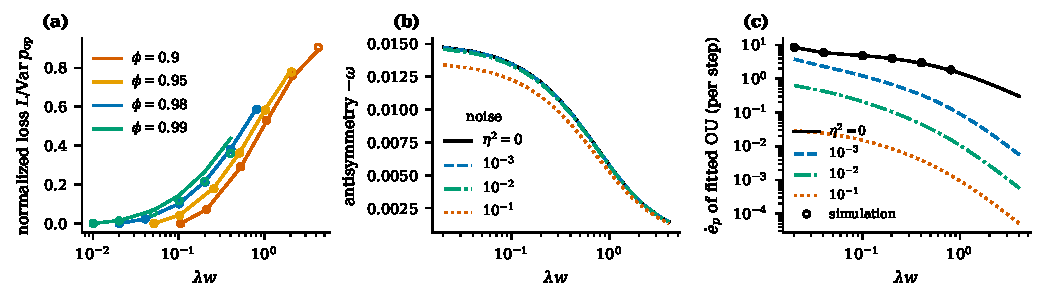
\includegraphics[width=\textwidth]{figures/fig2_gaussian_observer.pdf}
\caption{A reversible Ornstein--Uhlenbeck input seen through trailing windows $(w,4w)$ loses transition information and acquires a large fitted dissipation that is fixed by innovation geometry, not by the current. (a) Normalized compression loss of a threshold forecast (threshold $2\sigma$, horizon 10): lines, Eq.~\eqref{eq:mehler}; circles, Monte Carlo loss of the exact Bayes observer. (b) Lag-one antisymmetry for independent observation noise $\eta^2$ (relative to the window variance); it changes only through the noise-inflated variances. (c) Entropy production of the fitted OU model for the same noise levels; circles, simulation without noise.}
\label{fig:gauss}
\end{figure*}

\subsection{Double well: two rates}\label{sec:dw}

In a double well the compression term is governed by two rates: the local curvature within wells and the Kramers rate between them. The test system is $dx=-(x^3-x-c_t)\,dt+0.72\,dW^{(x)}$, $dc=-c\,\tau_c^{-1}dt+0.18\,dW^{(c)}$ with $\tau_c\in\{5,20,80,\infty\}$ ($c\equiv0$ for $\tau_c=\infty$), integrated with Euler steps of $0.05$; the event is $x\ge0.65$ within two time units, scored from states with $x<0.65$, and the oracle $\pOp(x,c)$ follows from the known generator. This is the textbook model of bifurcation- and noise-induced tipping \cite{ashwin2012}. The observer sees trailing means of $x$ and $c$ over $w$ steps. We estimate $L$ directly as the out-of-sample mean squared residual of a flexible regression of $\pOp$ on the observation, trained on $7\times10^5$ steps; at $w=1$ the estimate is below $10^{-3}$ (Appendix~\ref{app:tworate}).

A single-rate Gaussian theory with the local stiffness $\bar\lambda=\E[U''(x_L)]\simeq2$ predicts $\ell=s^2(\bar\lambda w)$ and overestimates the loss by between \SingleErrLo and \SingleErrHi [Fig.~\ref{fig:dw}(b)]. The reason is visible in the autocorrelation of $x$ [Fig.~\ref{fig:dw}(a)]: it decays with two rates, and the slow one ($0.169$) is the Kramers switching rate $\kappa=k_{L\to R}+k_{R\to L}=0.172$ \cite{kramers1940,hanggi1990}, not the curvature. The oracle inherits this structure: 85\% of $\mathrm{Var}\,\pOp$ lies between the two sides of the barrier and only 15\% within them, and a trailing window resolves the side for times shorter than $1/\kappa$. Splitting $\mathrm{Var}\,\pOp=V_b+V_w$ by the side and weighting each part by the posterior variance of its own rate gives the two-rate approximation
\begin{equation}
\ell(w)\simeq\frac{V_b\,s^2(\kappa w)+V_w\,s^2(\bar\lambda w)}{\mathrm{Var}\,\pOp},\label{eq:tworate}
\end{equation}
evaluated conditionally on $c$ for finite $\tau_c$, with Kramers rates of the tilted well and no fitted parameter. It reduces the error from between \SingleErrLo and \SingleErrHi to between \TwoErrLo and \TwoErrHi (Table~\Sref{dwloss}): the mechanism is right, and the remaining underestimate at the widest windows comes from hops inside the window, where the posterior of the side is far from Gaussian. The exact losses for the four control time scales nearly coincide at fixed $\bar\lambda w$. Estimating the same loss from the skill difference of a classifier trained on $8.4\times10^3$ points overstates it (\ClfEst against \ClfExact at $\tau_c=5$, $w=80$; Table~\Sref{dwloss}), because the classifier on wide windows loses skill to estimation rather than to compression.

\begin{figure*}[t]
\centering
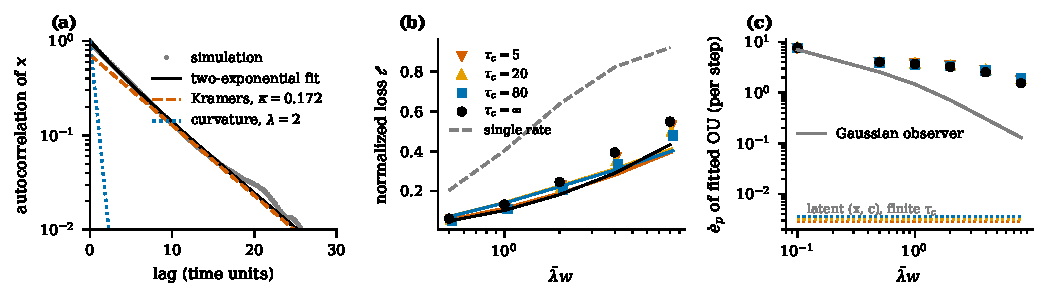
\includegraphics[width=\textwidth]{figures/fig3_double_well.pdf}
\caption{In the double well the loss is governed by two rates, and a two-window observer of a reversible well reports a large current. (a) Autocorrelation of $x$ for $\tau_c=\infty$: a fast intra-well part and a slow part decaying at the Kramers rate $\kappa$ (dashed), far from the curvature rate (dotted). (b) Normalized compression loss: markers, near-exact Bayes loss for four $\tau_c$; lines, two-rate approximation~\eqref{eq:tworate}; dashed, single-rate Gaussian theory. (c) Entropy production of the OU model fitted to two trailing windows $(w,4w)$ of $x$ alone (markers); dotted, the latent $(x,c)$ value for finite $\tau_c$; line, Gaussian observer with $\bar\lambda$ (Sec.~\ref{sec:gauss}).}
\label{fig:dw}
\end{figure*}

\section{Daily markets}\label{sec:market}

\subsection{Data, state and controls}\label{sec:data}

The early-warning state consists of seven trailing-window features of daily S\&P 500 prices and volumes, 3 January 2000 to 16 October 2026: log realized volatility over 20 and 5 days, relative log activity (20-day over 250-day mean volume), the 20-day drawdown and log return, and the rolling 60-day variance of the differenced and lag-one autocorrelation of log 20-day volatility, the standard critical-slowing-down indicators \cite{dakos2012}. Fitted to past data for forecasting, this state is reduced to its first two principal components [PCA(2)]. In the language of Proposition~\ref{prop:decomp} the inputs are the returns $r_t$, their squares and the volume; log volatilities over different windows are filters of one channel, whereas the return and the volatility over the same 20 days are filters of two channels with identical kernels.

Four controls rerun the whole feature pipeline on a modified input (Appendix~\ref{app:surrogates}). Time reversal of the returns and volumes gives $\omega^{\rm rev}$ and, through Eq.~\eqref{eq:estimator}, the two terms. Centered windows remove the observer term (Corollary~\ref{cor:symmetric}). Redrawing the signs of the actual returns removes the coupling between sign and future magnitude and keeps $|r_t|$. Reversible surrogates---an amplitude-adjusted Fourier transform \cite{schreiber1996} of $|r_t|$ with independent signs and phase-matched volume---keep the volatility clustering and are time reversible by construction; a version with symmetric signs removes the drift as well. Bitcoin and Ether states are built in the same way.

\begin{table*}[t]
\squeezetable
\caption{Lag-one antisymmetry of the market states and its decomposition, Eq.~\eqref{eq:estimator}. $\omega$, $\omega^{\rm rev}$ and $\omega^{\rm cen}$ are computed on features from the data, from the time-reversed input and with centered windows; $O=\tfrac12(\omega+\omega^{\rm rev})$, $P=\tfrac12(\omega-\omega^{\rm rev})$. In parentheses, moving-block-bootstrap standard errors in units of the last digit (20-day blocks, 1000 replicates, the three series resampled jointly; 60-day blocks in Table~\Sref{boot}). Surrogates: median [5\%, 95\%] of 200 (S\&P 500) or 100 (Bitcoin, Ether) reversible surrogates. The PCA(2) state is evaluated in the basis of the observed loadings. The centered drawdown is not a symmetric-kernel version of the trailing one (Sec.~\ref{sec:leverage}), so $\omega^{\rm cen}$ does not estimate $P$ in that row.}
\label{tab:markets}
\begin{ruledtabular}
\begin{tabular}{llrrrrrl}
 & channel & $\omega$ & $\omega^{\rm rev}$ & $\omega^{\rm cen}$ & $O$ & $P$ & surrogates\\
\hline
S\&P 500 & window & $-$0.0203(19) & $-$0.0202(21) & $+$0.0013(14) & $-$0.0202(17) & 0.0000(11) & $-$0.023 [$-$0.026, $-$0.020]\\
 & leverage, return & $+$0.0276(34) & $-$0.0276(35) & $+$0.0267(34) & 0.0000(28) & $+$0.0276(21) & 0.000 [$-$0.003, $+$0.004]\\
 & leverage, drawdown & $+$0.0221(30) & $-$0.0108(28) & $-$0.0018(32) & $+$0.0057(22) & $+$0.0165(18) & $+$0.003 [0.000, $+$0.006]\\
 & PCA(2) state & $+$0.0197(32) & $-$0.0206(29) & $+$0.0162(30) & $-$0.0004(25) & $+$0.0202(18) & $+$0.001 [$-$0.003, $+$0.004]\\
\hline
S\&P, to 2020 & window & $-$0.0189(22) & $-$0.0189(23) & $+$0.0004(16) & $-$0.0189(20) & 0.0000(12) & --\\
 & leverage, return & $+$0.0272(37) & $-$0.0263(37) & $+$0.0258(37) & $+$0.0005(28) & $+$0.0268(24) & --\\
 & PCA(2) state & $+$0.0173(29) & $-$0.0174(30) & $+$0.0153(30) & $-$0.0001(22) & $+$0.0174(19) & --\\
\hline
Bitcoin & window & $-$0.0271(28) & $-$0.0289(27) & $+$0.0049(26) & $-$0.0280(22) & $+$0.0009(16) & $-$0.029 [$-$0.033, $-$0.025]\\
 & leverage, return & $+$0.0039(41) & $-$0.0013(42) & $+$0.0041(41) & $+$0.0013(29) & $+$0.0026(30) & 0.000 [$-$0.004, $+$0.004]\\
 & PCA(2) state & $+$0.0049(34) & $+$0.0104(46) & $-$0.0078(40) & $+$0.0076(28) & $-$0.0028(30) & $+$0.007 [$+$0.002, $+$0.012]\\
\hline
Ether & window & $-$0.0309(29) & $-$0.0305(35) & $-$0.0011(33) & $-$0.0307(26) & $-$0.0002(19) & $-$0.036 [$-$0.042, $-$0.032]\\
 & leverage, return & $+$0.0012(36) & $+$0.0012(36) & $-$0.0007(39) & $+$0.0012(24) & 0.0000(27) & $+$0.001 [$-$0.005, $+$0.006]\\
 & PCA(2) state & $+$0.0051(31) & $+$0.0051(43) & $-$0.0095(43) & $+$0.0051(25) & 0.0000(28) & $+$0.006 [$+$0.001, $+$0.012]\\

\end{tabular}
\end{ruledtabular}

\end{table*}

\subsection{The window channel carries the observer term}\label{sec:window}

The volatility windows carry an observer term of the size found in time-reversible surrogates. For log realized volatility over 5 and 20 days the antisymmetry is \OmWinFwd for the data and for the time-reversed input alike, so it is entirely observer term ($|O|$ is \WinOz standard errors), and centering the windows removes it (Table~\ref{tab:markets}). Reversible surrogates, symmetric-sign surrogates and a stochastic-volatility model without leverage give values of the same size [Fig.~\ref{fig:market}(a)]. This is Corollary~\ref{cor:single} in data: the short window leads the long one whatever the direction of time. The OU model fitted to this pair reports $\dot e_p=\,$\EpWinObs per day, and the same model fitted to the surrogates \EpWinSurMed (median)---the large fitted dissipation of the Gaussian observer, now in a market.

\subsection{The leverage channel carries the physical term}\label{sec:leverage}

The physical term is the leverage effect: it reverses under time reversal, survives centering and vanishes when return signs are randomized. For the 20-day return against 20-day log volatility the antisymmetry is \OmLevFwd forward and \OmLevRev backward, so it is entirely physical ($P$ is \LevPz standard errors); it stays at \OmLevCen with centered windows and vanishes in the surrogates [Table~\ref{tab:markets}, Fig.~\ref{fig:market}(b)]. Both features have the same 20-day support, so their observer term vanishes identically (Corollary~\ref{cor:symmetric}); what remains is the odd part of the cross-covariance between returns and later squared returns, the leverage effect \cite{black1976,bouchaud2001} [Fig.~\ref{fig:decomp}(c)]. With linear windows of $r_t$ and $r_t^2$ the decomposition is exact: Proposition~\ref{prop:decomp} evaluated with the empirical cross-covariances reproduces every measured antisymmetry to four decimals in both directions of time (Table~\Sref{prop1}).

The 20-day drawdown, a running maximum and hence a strongly nonlinear filter, shows the limits of the centering control. Equation~\eqref{eq:estimator} attributes most of its antisymmetry with volatility to the physical term ($P=\,$\DDP, $O=\,$\DDO). The centered drawdown, $c_t/\max_{|k|\le10}c_{t+k}-1$, is not a symmetric-kernel version of the trailing one: it responds to losses before $t$ and to gains after $t$ alike, so the two orientations of its lead--lag relation with volatility nearly cancel ($\omega^{\rm cen}=\,$\DDCen). Centering removes the observer term only for features whose centered version is the same functional with a symmetric kernel, whereas time reversal needs no such assumption.

\subsection{What the forecasting state sees}\label{sec:pca}

The forecasting state sees mostly the physical term, because its two leading components discard the direction in which the observer term lives. In the basis of the observed loadings the PCA(2) antisymmetry is \OmPcaFwd forward and \OmPcaRev backward, so the observer term is negligible ($O=\,$\OPcaRev, while $P$ is \PcaPz standard errors); centered windows keep most of it (\OmPcaCen), and the surrogates give zero [Fig.~\ref{fig:market}(c)]. The centering estimate of the observer term, $\omega-\omega^{\rm cen}=\,$\OPcaCen, differs from the time-reversal estimate because the state loads on the drawdown (weights \DDLoadOne and \DDLoadTwo on the two components), whose centered version fails as a control (Sec.~\ref{sec:leverage}). Its fitted entropy production is \EpPca per day, against a median of \EpSurMed, a 95th percentile of \EpSurQ and a maximum of \EpSurMax for the \NSur reversible surrogates (Table~\Sref{surr}): the observed value is \EpObsOverMax times the largest surrogate value. By Proposition~\ref{prop:factor} the excess is a current, not a geometry effect: $\omega_{\rm fit}^2$ is \OmFitSqRatio times and $\mathcal G$ only \GRatio times its surrogate median. The observer term is absent because both volatility features load on the first component with the same sign; their difference, in which the window current lives, falls into a discarded component. Re-fitting the principal components on time-reversed features shows why the size of $\dot e_p$ alone can mislead. The re-fitted plane differs from the observed one, and in it $|\omega_{\rm fit}|=\,$\OmFitRevRefit instead of \OmFitPca while $\mathcal G=\,$\GRevRefit instead of \GPca, so $\dot e_p=\,$\EpRevRefit against \EpPca forward; in the fixed basis of the observed loadings the reversed state has $|\omega_{\rm fit}|=\,$\OmFitRevFixed and $\dot e_p=\,$\EpRevFixed, close to the forward values. By Proposition~\ref{prop:factor} the change lies in the current within a different plane, not in the geometry factor. Every signed comparison is therefore made in one fixed basis.

\begin{figure*}[t]
\centering
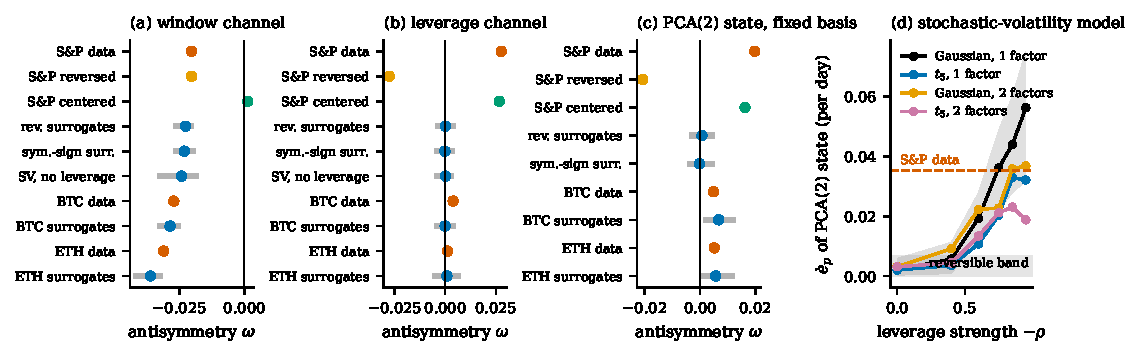
\includegraphics[width=\textwidth]{figures/fig4_markets.pdf}
\caption{In daily markets the volatility windows carry the observer term and the leverage effect carries the physical term. (a) Window channel (log realized volatility over 5 and 20 days): data, time-reversed and centered inputs (colored), reversible and symmetric-sign surrogates, a stochastic-volatility model without leverage, Bitcoin and Ether (median and 5--95\% range for ensembles). (b) Leverage channel (20-day return and 20-day log volatility). (c) PCA(2) forecasting state in the basis of the observed loadings. (d) Entropy production of the PCA(2) state of the stochastic-volatility model against leverage strength for four variants (band: 5--95\% for the Gaussian one-factor model), the S\&P 500 value (dashed) and the reversible-surrogate band (gray).}
\label{fig:market}
\end{figure*}

\subsection{A generative check}\label{sec:sv}

A stochastic-volatility model reproduces the window-channel term and, with leverage, brackets the physical one. Returns are $r_t=e^{h_t/2}\varepsilon_t$ with an autoregressive log variance whose shocks correlate with the previous return shock with coefficient $\rho$ \cite{harvey1996}; the persistence and the coupling of volume to volatility are calibrated to the data, with Gaussian or Student-$t$ shocks and one or two volatility factors (Appendix~\ref{app:data}). Without leverage ($\rho=0$) the median PCA(2) entropy production of every variant lies inside the reversible band and its 95th percentile does not exceed \SVQnfMax, while the full window-channel current is present (Table~\ref{tab:sv}). With leverage strong enough to reproduce the leverage-channel antisymmetry of the data (\OmLevData; medians interpolated in $\rho$), the PCA(2) entropy production is \SVMatchLo--\SVMatchHi per day across variants, bracketing the observed \EpPca [Fig.~\ref{fig:market}(d)]; the Student-$t$ one-factor model reaches at most $\omega_{\rm lev}=\,$\TOneLevMax, where $\dot e_p=\,$\TOneEpAtMax. At $\rho=-0.95$ the Gaussian two-factor model also reproduces the leverage sum $L_+=\sum_{k=1}^{20}\langle r_tr_{t+k}^2\rangle/\langle r_t^2\rangle^2$ of the data. The models bracket the observed values but do not pin them down.

\begin{table}[t]
\caption{Stochastic-volatility null for the PCA(2) state: median entropy production per day, leverage-channel antisymmetry and leverage sum $L_+$ for 30 replicates per leverage coefficient $\rho$, for the simplest and the richest variant (all four in Table~\Sref{sv}).}
\label{tab:sv}
\begin{ruledtabular}
\begin{tabular}{rrrrrrr}
 & \multicolumn{3}{c}{Gaussian, one factor} & \multicolumn{3}{c}{Student-$t$, two factors}\\
$\rho$ & $\dot e_p$ & $\omega_{\rm lev}$ & $L_+$ & $\dot e_p$ & $\omega_{\rm lev}$ & $L_+$\\
\hline
0.00 & 0.0020 & $+$0.0005 & $-$11 & 0.0031 & 0.0000 & 9\\
$-$0.40 & 0.0057 & $+$0.0123 & $-$109 & 0.0044 & $+$0.0139 & $-$176\\
$-$0.60 & 0.0193 & $+$0.0179 & $-$207 & 0.0134 & $+$0.0224 & $-$242\\
$-$0.75 & 0.0362 & $+$0.0243 & $-$222 & 0.0212 & $+$0.0255 & $-$346\\
$-$0.85 & 0.0440 & $+$0.0268 & $-$260 & 0.0231 & $+$0.0287 & $-$337\\
$-$0.95 & 0.0564 & $+$0.0301 & $-$295 & 0.0188 & $+$0.0312 & $-$363\\
\hline
data & 0.0352 & $+$0.0276 & $-$397 & \multicolumn{3}{c}{(same)}\\
\end{tabular}
\end{ruledtabular}

\end{table}

\subsection{Other samples and higher orders}\label{sec:robust}

The split repeats on the 2000--2020 subsample (Table~\ref{tab:markets}). Bitcoin and Ether carry even stronger observer terms in the window channel but no leverage ($|P|\le\,$\CryptoPmax, in the leverage channel less than one standard error); accordingly their PCA(2) states, whose small antisymmetry is mostly observer made, lie inside their reversible bands. Corollary~\ref{cor:single} also marks what second-order window statistics cannot see. The volatility series itself is time asymmetric at third order: the Ramsey--Rothman-type statistic $\sum_{k\le20}\langle z_t^2z_{t+k}-z_tz_{t+k}^2\rangle$ of $z=|r_t|$ is \RRobs, outside the amplitude-adjusted-surrogate range [\RRlo, \RRhi] ($p=\,$\RRp; Table~\Sref{third}) \cite{ramsey1996}. Yet the window channel built from $|r_t|$ is the same forward and backward, as it must be.

\subsection{What the windows cost in information}\label{sec:mktinfo}

The information loss of Sec.~\ref{sec:info} has a market reading. The one-factor stochastic-volatility model calibrated to the autocorrelation of log 20-day volatility (Appendix~\ref{app:data}) relaxes at $\lambda=\,$\LamMkt per day, so the market's 5- and 20-day volatility windows are the first row of Table~\ref{tab:gauss}: even if they averaged the latent log variance itself, they would lose $\ell=\,$\EllMktPair of the information it carries about an excursion beyond $2\sigma$ within ten days, and single windows of 20, 60 and 250 days would lose \EllWinTwenty, \EllWinSixty and \EllWinTwoFifty (Lemma~\ref{lem:mehler}, Table~\Sref{mktinfo}). The pipeline's windows average squared returns instead, a noisy proxy of the variance. In $10^6$-day simulations of the calibrated model the pair of log realized volatilities loses $\ell=\,$\EllMktRV and the PCA(2) state \EllMktPca, estimated as the out-of-sample error of a flexible regression of the oracle on the observation; the same estimator recovers the exact loss of the noise-free pair to within \EllCheckDiff. Most of what the forecasting state does not know about the next volatility excursion is therefore lost to the noise of its inputs rather than to the delay of the windows, and no estimator built on that state can recover it.


\section{Discussion}\label{sec:discussion}

The size of a fitted entropy production says little by itself. The fitted OU model is misspecified---a windowed state is not Markov---but it is the model that windowed early-warning pipelines fit, and Proposition~\ref{prop:factor} separates its current, measured by $\omega_{\rm fit}$, from the innovation geometry, measured by $\mathcal G$. The latter can vary by orders of magnitude between states with similar currents: for the Gaussian observer with noise-free windows $\mathcal G$ exceeds $10^4$, whereas in the market forecasting state it is \GPca, and re-fitting a reduction can change $\dot e_p$ several-fold without any change in the dynamics (Sec.~\ref{sec:pca}). Reporting $\omega$ alongside $\dot e_p$ makes such numbers comparable.

Irreversibility measured on windows of one observable is a property of the windows (Corollary~\ref{cor:single}). Second-order indicators built from several trailing windows of a single signal cannot distinguish a reversible from an irreversible system; detecting the latter requires higher-order statistics or genuinely distinct observed channels. For multichannel states the time-reversed data provide a model-free baseline, because the observer term is what survives reversal, and centered windows provide a second one where the features allow it. When irreversibility is used as an early-warning signal \cite{kooloth2026,xu2023} on states assembled from trailing features, the observer term should be removed first; Eq.~\eqref{eq:estimator} costs one extra pass of the feature pipeline.

In financial data the two terms have distinct origins. The observer term lives in comparisons of volatility over different windows and is present at full strength in surrogates whose volatility dynamics is reversible. The physical term is the odd part of the cross-covariance between signed returns and later volatility, the leverage effect; it survives centered windows and disappears with random signs. Higher-order asymmetry of volatility itself, the Zumbach effect \cite{zumbach2009,lynch2003}, exists in the same data (Sec.~\ref{sec:robust}) but is invisible to second-order window statistics. This is consistent with the finding that time-reversal violations of returns measured through feedback kernels reflect the ARCH mechanism rather than leverage \cite{chicheportiche2014}: that statistic is of higher order, ours is of second order, and the two probe different channels.

For information loss the lesson is that the relevant clock is the slowest relaxation, not the local one. In the double well most of the oracle's variance lies between the wells and decorrelates at the Kramers rate, so trailing windows much longer than the local relaxation time still preserve most of the transition information; a single-rate theory based on local curvature overestimates the loss by a factor of \SingleFacLo to \SingleFacHi. In the market the windows themselves are not the main loss: averaging the latent variance, the 5- and 20-day windows would lose \EllMktPair of the information about the next volatility excursion, but they average squared returns and lose \EllMktRV (Sec.~\ref{sec:mktinfo}). Forecasts that integrate a fitted drift, such as committor-type hitting probabilities, inherit both effects of the observer; a companion paper evaluates such forecasts on the same market state \cite{xing2026b}.

The study has limits. Proposition~\ref{prop:decomp} is exact for linear filters and second-order statistics; for nonlinear features such as running maxima the split is approximate and the centering control fails, and higher-order irreversibility is outside its scope. The empirical part rests on one equity index and two cryptocurrencies at daily sampling. The stochastic-volatility check uses one- and two-factor models, which bracket but do not pin down the observed values, and the market reading of the information loss rests on the one-factor calibration. The two-rate approximation for the double well captures the mechanism but underestimates the loss at the widest windows by up to \TwoErrAbs.

\section{Conclusion}\label{sec:conclusion}

Trailing windows add a current of their own to whatever current a system carries; at second order the two separate exactly under time reversal, and the same windows destroy transition information at rates set by the system's relaxation, including Kramers switching in metastable systems. For an Ornstein--Uhlenbeck input both effects are in closed form, and the large fitted dissipation of reversible inputs is a geometric consequence of collinear innovations. In daily S\&P 500 data the volatility windows carry the observer's current and the leverage effect carries the physical one, and the forecasting state lacks about half of the information that the latent volatility carries about its next excursion. The same accounting applies to any early-warning state built from windows, for instance in climate and ecological indicators.


\begin{acknowledgments}
We used AI assistants, including Claude (Anthropic), to develop analysis code and to edit the text; every numerical result was produced by the deposited, seeded scripts, which the authors ran and checked, and the authors take full responsibility for the content.
\end{acknowledgments}

\emph{Data and code availability.} Data snapshots, scripts, all intermediate tables, figures and SHA-256 manifests are deposited at \url{https://github.com/SavitAR296/committor-market-transition-benchmark} (directory \nolinkurl{paper1_pre/}, commit \RepoCommit) and archived on Zenodo (DOI \ZenodoDOI); every result number in the text is generated as a macro with its source table, and Table~\Sref{files} of the Supplemental Material \cite{SM} lists the files behind each figure and table.

\appendix

\section{Gaussian observer}\label{app:gauss}

\emph{Covariances.} For trailing means $y_i(t)=w_i^{-1}\sum_{a=0}^{w_i-1}x_{t-a}$ of a stationary AR(1) with $r(k)=\phi^{|k|}$,
\begin{equation}
C_{ij}(s)=\frac{1}{w_iw_j}\sum_{a=0}^{w_i-1}\sum_{b=0}^{w_j-1}\phi^{|s-a+b|},\qquad c_i=\frac{1-\phi^{w_i}}{w_i(1-\phi)},
\end{equation}
$c_i=\mathrm{Cov}(x_t,y_i(t))$. In continuous time the double integral of $e^{-\lambda|s-a+b|}$ equals $F(s+w_j)-F(s)-F(s-w_i+w_j)+F(s-w_i)$ with $F(u)=(e^{-\lambda|u|}+\lambda|u|)/\lambda^2$, the second antiderivative of $e^{-\lambda|u|}$, and $c_i=(1-e^{-\lambda w_i})/(\lambda w_i)$. Ten simulations of $10^6$ steps reproduce $C(0)$, $C(1)$ and $C(5)$ to $0.07\%$ (Table~\Sref{gauss} \cite{SM}). Since $\phi^{|k|}$ is even, Proposition~\ref{prop:decomp} gives $\omega=O$, and the closed form of $\omega$ in Table~\ref{tab:gauss} follows from $C(1)$.

\emph{Exact information loss.} Let $\beta=C(0)^{-1}c$, $m=\beta^\top y$ and $s^2=1-c^\top C(0)^{-1}c$. Then $x_t\mid y_t\sim N(m,s^2)$, independent of the observed value, and $(x_t,m/\sqrt{1-s^2})$ is a standard bivariate normal pair with correlation $\rho=\sqrt{1-s^2}$. Mehler's formula $\E[h_n(X)\mid M]=\rho^nh_n(M)$ for the orthonormal Hermite polynomials $h_n$ \cite{mehler1866,odonnell2014} gives $r^*(y)=\sum_na_n\rho^nh_n(M)$, hence $\E[r^{*2}]=\sum_na_n^2(1-s^2)^n$ and, with $\E[(r^*-\pOp)^2]=\E[\pOp^2]-\E[r^{*2}]$, Eq.~\eqref{eq:mehler}. Every term increases with $s^2$, $L(0)=0$, $L(1)=\mathrm{Var}\,\pOp$, and $L'(0)=\sum_n na_n^2=\E[\pOp'(X)^2]$. For the AR(1) threshold events the series and a direct two-dimensional quadrature agree to $10^{-6}$. The oracle $\pOp$ is the first-passage probability from a backward recursion with exact Gaussian cell probabilities.

\emph{Singularity and noise.} The window transfer functions are $K_i(\omega)=e^{-i\omega(w_i-1)/2}\sin(\omega w_i/2)/[w_i\sin(\omega/2)]$, a real amplitude times a delay of $(w_i-1)/2$ steps. The spectral matrix $S_x(\omega)K(\omega)K(\omega)^\dagger$ has rank one; the forward process obeys the exact relation $K_2(L)y_1=K_1(L)y_2$ in the lag operator $L$ and the reversed one does not, so the path measures are mutually singular. Independent noise of variance $\eta^2$ makes the spectral matrix invertible and the divergence rate finite, growing as $\eta^{-2}$; in Eq.~\eqref{eq:factor} the same noise lifts $d_{\min}$ by $O(\eta^2)$.

\emph{Fitted model.} With $A\Sigma=-\tfrac12D+\Omega$, the Fokker--Planck current of the fitted OU is $J=Ay\rho-\tfrac12D\nabla\rho=\Omega\Sigma^{-1}y\rho$, and $\dot e_p=\int J^\top(\tfrac12D)^{-1}J\rho^{-1}dy$ gives Eq.~\eqref{eq:ep}. The Markov divergence between forward and backward pairs is $d_1=\tfrac12[\mathrm{tr}(\Gamma_r^{-1}\Gamma)-2m]$ with $\Gamma=\bigl(\begin{smallmatrix}C(0)&C(1)^\top\\C(1)&C(0)\end{smallmatrix}\bigr)$ and $\Gamma_r$ its block transpose. Proposition~\ref{prop:factor} follows from $\Omega=\omega_{\rm fit}\mathsf J$ and $\mathsf J^\top D^{-1}\mathsf J=D/\det D$; Eq.~\eqref{eq:factor} holds to $4\times10^{-15}$ on every configuration of Table~\Sref{factor}.

\section{Physical current of one-way slow driving}\label{app:oneway}

The control for an observer-induced current is the current of a latent process that is genuinely driven. For $dx=(-\lambda x+c)\,dt+\sqrt{2\lambda}\,dW_1$, $dc=-\mu c\,dt+\sigma_c\,dW_2$, i.e.\ $A=\bigl(\begin{smallmatrix}-\lambda&1\\0&-\mu\end{smallmatrix}\bigr)$, $D=\mathrm{diag}(2\lambda,\sigma_c^2)$, the Lyapunov equation gives $\Sigma_{cc}=\sigma_c^2/(2\mu)$, $\Sigma_{xc}=\Sigma_{cc}/(\lambda+\mu)$, $\Sigma_{xx}=1+\Sigma_{xc}/\lambda$, the antisymmetric part $\omega=\sigma_c^2/[2(\lambda+\mu)]$ and
\begin{equation}
\dot e_p=\frac{2\omega^2}{\det\Sigma}\Big(\frac{\Sigma_{cc}}{\sigma_c^2}+\frac{\Sigma_{xx}}{2\lambda}\Big)\ \xrightarrow{\ \mu\to0\ }\ \frac{\sigma_c^2}{2\lambda^2}.
\end{equation}
For $\lambda=2$ and $\sigma_c=0.18$ this is $3.7\times10^{-3}$ at $1/\mu=5$ and $4.05\times10^{-3}$ for $\mu\to0$; exact-discretization simulations recover these values within 2--14\%. At fixed $\sigma_c$ a slow driver does not make the latent dynamics reversible; only $\sigma_c=0$ does, which is why the double well with $c\equiv0$ is the clean control of Sec.~\ref{sec:dw}.

\section{Two-rate approximation for the double well}\label{app:tworate}

\emph{Rates.} For $U(x;c)=x^4/4-x^2/2-cx$ with stationary points $x_L<x_0<x_R$, Kramers' formula \cite{kramers1940,hanggi1990} gives $k_{L\to R}=\sqrt{U''(x_L)|U''(x_0)|}\,e^{-[U(x_0)-U(x_L)]/D}/(2\pi)$ and similarly $k_{R\to L}$, with $D=\sigma_x^2/2$. The side of the barrier then follows a telegraph process whose autocorrelation decays at $\kappa=k_{L\to R}+k_{R\to L}$; within a side the state relaxes at the curvature $\lambda=U''(x_L)$. For $c=0$, $\kappa=0.172$, and a two-exponential fit to the simulated autocorrelation of $x$ gives a slow rate of $0.169$ with weight $0.71$ [Fig.~\ref{fig:dw}(a)].

\emph{Approximation.} By the law of total variance over the side $B$, $\mathrm{Var}\,\pOp=V_b+V_w$ with $V_b=\pi_L\pi_R(\bar p_R-\bar p_L)^2$, where $\pi_k$ and $\bar p_k$ are the occupation and mean oracle of side $k$, and $V_w$ the mean within-side variance. Each part is weighted by the posterior variance of a unit OU process of its own rate given a trailing mean of $w$ steps of spacing $\Delta$,
\begin{align}
s^2(r)&=1-\frac{\bar c(r)^2}{V(r)},\qquad \bar c(r)=\frac{1}{w}\sum_{a}e^{-ra\Delta},\nonumber\\
V(r)&=\frac{1}{w^2}\sum_{a,b}e^{-r|a-b|\Delta},
\end{align}
which gives Eq.~\eqref{eq:tworate}. For finite $\tau_c$ the construction is applied in twelve quantile bins of $c$, with rates and variances evaluated in each bin, and averaged; this treats $c$ as known, which is accurate when $w\ll\tau_c$. Bins beyond the fold of the tilted well (one minimum) use the curvature channel only. The approximation has no fitted parameter. It neglects that a hop inside the window makes the posterior of the side bimodal; a Gaussian-copula treatment of the side, which we also tried, overestimates the loss for the opposite reason---the side is a deterministic function of the current state, not a noisy Gaussian channel.

\emph{Near-exact loss.} $L(w)=\E[\mathrm{Var}(\pOp\mid\bar x_w,\bar c_w)]$ is the out-of-sample mean squared residual of a gradient-boosted regression of $\pOp$ on the observation, trained on the first 60\% of a $1.2\times10^6$-step path; at $w=1$, where the observation determines $\pOp$, it is below $10^{-3}$, and for $\tau_c=\infty$ it agrees with a 400-bin conditional variance to $0.013$.

\section{Controls and surrogates}\label{app:surrogates}

Every control reruns the full feature pipeline on a modified input. \emph{Time reversal}: the log-return and volume sequences are reversed and prices rebuilt by cumulation. \emph{Centered windows}: symmetric windows of 5, 21, 61 and 251 days replace the trailing ones, the 20-day return becomes $\log c_{t+10}-\log c_{t-10}$ and the drawdown $c_t/\max_{|k|\le10}c_{t+k}-1$. \emph{Random signs}: the signs of the actual returns are redrawn independently with the empirical up-probability, keeping $|r_t|$ and volume; this removes the sign--magnitude coupling and keeps any asymmetry of $|r_t|$ itself. \emph{Reversible surrogates}: an iterated amplitude-adjusted Fourier transform \cite{schreiber1996} of $|r_t|$ with independent signs; log volume receives the same random phases with a symmetrized cross-spectrum and is rank-remapped to its marginal. \emph{Symmetric-sign surrogates}: as before with signs of probability $1/2$, which removes the drift and makes the input strictly time reversible. A single zero volume is enough to break this construction silently: $\log 0=-\infty$ turns the volume Fourier transform into undefined numbers, after which the volume phases no longer depend on the random seed and every surrogate shares one volume path. Yahoo's \textasciicircum{}GSPC record contains such a day (24 May 2023); a data gate rejects non-positive volumes, and the day is filled from a second vendor before any analysis (Appendix~\ref{app:data}).

\section{Data, features and the stochastic-volatility model}\label{app:data}

\emph{Data.} S\&P 500: vega-datasets snapshot of Yahoo Finance \textasciicircum{}GSPC daily data, 3 January 2000 to 17 April 2020, continued to 16 October 2026 with \textasciicircum{}GSPC daily data downloaded in October 2026 through Yahoo's chart interface. On the 326 days shared by the two sources (2019--2020) the closes coincide; Yahoo has since revised the volume of 27 of those days by more than 1\% (median ratio 0.997). The snapshot also agrees with an independent Yahoo-derived archive \cite{vijinho} on all 4774 common days to 21 December 2018 (closes to a relative $5.7\times10^{-8}$, volumes to $0.08\%$). Yahoo's record has volume zero on 24 May 2023; we fill it with the $3.739\times10^9$ shares ($3739.16\times10^4$ lots of 100 shares) reported by a second vendor, Tonghuashun, whose open, high, low and close for that day and whose volumes on the two adjacent days coincide with Yahoo's. Replacing it by the mean volume of the adjacent days (\VolAdj shares) changes no entry of Table~\ref{tab:markets} at the precision shown and no fitted quantity by more than \VolMaxDiff. Bitcoin and Ether: Coin Metrics community data from 1 January 2013 and 1 March 2016.

\emph{Features.} Log 20-day and 5-day realized volatility, relative log activity (20-day over 250-day mean volume), 20-day drawdown, 20-day log return, and the rolling 60-day variance of the differenced and lag-one autocorrelation of log 20-day volatility \cite{dakos2012}. The forecasting state is the first two principal components of the standardized features, re-standardized. Because principal axes have arbitrary signs, all signed antisymmetries of the principal-component state are computed in the basis of the observed loadings with PC1 oriented to load positively on log 20-day volatility and PC2 on the rolling variance; only $\dot e_p$, $|\omega|$ and $\mathcal G$ are basis independent.

\emph{Stochastic-volatility model.} $r_t=e^{h_t/2}\varepsilon_t$ with $h_t=\mu+\sum_jh^{(j)}_t$, $h^{(j)}_t=\phi_jh^{(j)}_{t-1}+s_j\eta^{(j)}_t$ and $\eta^{(j)}_t=\rho\,\varepsilon_{t-1}+\sqrt{1-\rho^2}\,\xi^{(j)}_t$, the asymmetric (leverage) form \cite{harvey1996}; $\varepsilon_t$ is standard normal or unit-variance Student-$t$ with five degrees of freedom. One factor: $\phi=0.98$; two factors: $\phi=(0.90,0.995)$ with equal variance shares, chosen from a grid by the autocorrelation of log 20-day volatility at lags 20, 60, 120 and 250. Total variances match the standard deviation of log 20-day volatility in the data ($0.50$), and the mean matches the return variance. Volume is $\log v_t=\mathrm{const}+\kappa(h_t-\mu)/2+\zeta_t$ with $\zeta$ an AR(1); $\kappa=0.19$, coefficient $0.60$ and innovation standard deviation $0.16$ are the regression of detrended log volume on detrended log 20-day volatility in the data and the AR(1) fit of its residual.


\begin{thebibliography}{99}
\bibitem{scheffer2009} M. Scheffer, J. Bascompte, W. A. Brock, V. Brovkin, S. R. Carpenter, V. Dakos, H. Held, E. H. van Nes, M. Rietkerk, and G. Sugihara, Nature \textbf{461}, 53 (2009).
\bibitem{kuehn2011} C. Kuehn, Physica D \textbf{240}, 1020 (2011).
\bibitem{dakos2012} V. Dakos, S. R. Carpenter, W. A. Brock, A. M. Ellison, V. Guttal, A. R. Ives, S. K\'efi, V. Livina, D. A. Seekell, E. H. van Nes, and M. Scheffer, PLoS ONE \textbf{7}, e41010 (2012).
\bibitem{lenton2012} T. M. Lenton, V. N. Livina, V. Dakos, E. H. van Nes, and M. Scheffer, Phil. Trans. R. Soc. A \textbf{370}, 1185 (2012).
\bibitem{kooloth2026} P. Kooloth, J. Lu, A. Rupe, D. DeSantis, and C. Bakker, Commun. Earth Environ. \textbf{7}, 250 (2026).
\bibitem{koolothcode2025} P. Kooloth \textit{et al.}, Code repository for ``Time irreversibility as an indicator of approaching tipping points in Earth subsystems,'' Zenodo record 17904887 (2025), \doi{10.5281/zenodo.17904887}.
\bibitem{xu2023} L. Xu, D. Patterson, S. A. Levin, and J. Wang, Proc. Natl. Acad. Sci. U.S.A. \textbf{120}, e2218663120 (2023).
\bibitem{xing2026b} B. Xing and J. Pan, What does a committor score forecast? Hitting-probability warnings of market stress, their target and their evaluation, submitted to Int. J. Forecast. (2026).% replace by the arXiv identifier once posted
\bibitem{boettiger2012} C. Boettiger and A. Hastings, J. R. Soc. Interface \textbf{9}, 2527 (2012).
\bibitem{ditlevsen2010} P. D. Ditlevsen and S. J. Johnsen, Geophys. Res. Lett. \textbf{37}, L19703 (2010).
\bibitem{duplessis2026} F. Du Plessis, V. Volodina, C. A. Boulton, M. Fadera, S. Kachhara, T. M. Lenton, P. D. L. Ritchie, and P. Ashwin, arXiv:2610.01677.
\bibitem{martinez2019} I. A. Mart\'inez, G. Bisker, J. M. Horowitz, and J. M. R. Parrondo, Nat. Commun. \textbf{10}, 3542 (2019).
\bibitem{hartich2024} D. Hartich and A. Godec, Nat. Commun. \textbf{15}, 8678 (2024).
\bibitem{bisker2024} G. Bisker, I. A. Mart\'inez, J. M. Horowitz, and J. M. R. Parrondo, Nat. Commun. \textbf{15}, 8679 (2024).
\bibitem{esposito2012} M. Esposito, Phys. Rev. E \textbf{85}, 041125 (2012).
\bibitem{lucente2022prr} D. Lucente, A. Baldassarri, A. Puglisi, A. Vulpiani, and M. Viale, Phys. Rev. Res. \textbf{4}, 043103 (2022).
\bibitem{bgjs2015} N. Barberis, R. Greenwood, L. Jin, and A. Shleifer, J. Financ. Econ. \textbf{115}, 1 (2015).
\bibitem{daw2000} C. S. Daw, C. E. A. Finney, and M. B. Kennel, Phys. Rev. E \textbf{62}, 1912 (2000).
\bibitem{porta2008} A. Porta, K. R. Casali, A. G. Casali, T. Gnecchi-Ruscone, E. Tobaldini, N. Montano, S. Lange, D. Geue, D. Cysarz, and P. Van Leeuwen, Am. J. Physiol. Regul. Integr. Comp. Physiol. \textbf{295}, R550 (2008).
\bibitem{lacasa2012} L. Lacasa, A. Nu\~nez, \'E. Rold\'an, J. M. R. Parrondo, and B. Luque, Eur. Phys. J. B \textbf{85}, 217 (2012).
\bibitem{flanagan2016} R. Flanagan and L. Lacasa, Phys. Lett. A \textbf{380}, 1689 (2016).
\bibitem{zanin2021} M. Zanin and D. Papo, Entropy \textbf{23}, 1474 (2021).
\bibitem{weiss1975} G. Weiss, J. Appl. Probab. \textbf{12}, 831 (1975).
\bibitem{tong2005} H. Tong and Z. Zhang, Stat. Sin. \textbf{15}, 495 (2005).
\bibitem{chan2006} K.-S. Chan, L.-H. Ho, and H. Tong, Biometrika \textbf{93}, 221 (2006).
\bibitem{ghanta2017} A. Ghanta, J. C. Neu, and S. Teitsworth, Phys. Rev. E \textbf{95}, 032128 (2017).
\bibitem{gonzalez2019} J. P. Gonzalez, J. C. Neu, and S. W. Teitsworth, Phys. Rev. E \textbf{99}, 022143 (2019).
\bibitem{gradziuk2019} G. Gradziuk, F. Mura, and C. P. Broedersz, Phys. Rev. E \textbf{99}, 052406 (2019).
\bibitem{battle2016} C. Battle, C. P. Broedersz, N. Fakhri, V. F. Geyer, J. Howard, C. F. Schmidt, and F. C. MacKintosh, Science \textbf{352}, 604 (2016).
\bibitem{roldan2010} \'E. Rold\'an and J. M. R. Parrondo, Phys. Rev. Lett. \textbf{105}, 150607 (2010).
\bibitem{roldan2012} \'E. Rold\'an and J. M. R. Parrondo, Phys. Rev. E \textbf{85}, 031129 (2012).
\bibitem{skinner2021} D. J. Skinner and J. Dunkel, Proc. Natl. Acad. Sci. U.S.A. \textbf{118}, e2024300118 (2021).
\bibitem{harunari2022} P. E. Harunari, A. Dutta, M. Polettini, and \'E. Rold\'an, Phys. Rev. X \textbf{12}, 041026 (2022).
\bibitem{vandermeer2022} J. van der Meer, B. Ertel, and U. Seifert, Phys. Rev. X \textbf{12}, 031025 (2022).
\bibitem{teza2020} G. Teza and A. L. Stella, Phys. Rev. Lett. \textbf{125}, 110601 (2020).
\bibitem{zumbach2009} G. Zumbach, Quant. Finance \textbf{9}, 505 (2009).
\bibitem{lynch2003} P. E. Lynch and G. O. Zumbach, Quant. Finance \textbf{3}, 320 (2003).
\bibitem{chicheportiche2014} R. Chicheportiche and J.-P. Bouchaud, Physica A \textbf{410}, 174 (2014).
\bibitem{black1976} F. Black, in \textit{Proceedings of the 1976 Meetings of the Business and Economic Statistics Section} (American Statistical Association, Washington, DC, 1976), p.~177.
\bibitem{bouchaud2001} J.-P. Bouchaud, A. Matacz, and M. Potters, Phys. Rev. Lett. \textbf{87}, 228701 (2001).
\bibitem{slutzky1937} E. Slutzky, Econometrica \textbf{5}, 105 (1937).
\bibitem{seifert2012} U. Seifert, Rep. Prog. Phys. \textbf{75}, 126001 (2012).
\bibitem{SM} See Supplemental Material at [URL will be inserted by publisher] for Tables S1--\Sref{files}.
\bibitem{murphy1973} A. H. Murphy, J. Appl. Meteorol. \textbf{12}, 595 (1973).
\bibitem{degroot1983} M. H. DeGroot and S. E. Fienberg, The Statistician \textbf{32}, 12 (1983).
\bibitem{brocker2009} J. Br\"ocker, Q. J. R. Meteorol. Soc. \textbf{135}, 1512 (2009).
\bibitem{mehler1866} F. G. Mehler, J. Reine Angew. Math. \textbf{66}, 161 (1866).
\bibitem{odonnell2014} R. O'Donnell, \textit{Analysis of Boolean Functions} (Cambridge University Press, Cambridge, 2014).
\bibitem{ashwin2012} P. Ashwin, S. Wieczorek, R. Vitolo, and P. Cox, Phil. Trans. R. Soc. A \textbf{370}, 1166 (2012).
\bibitem{kramers1940} H. A. Kramers, Physica \textbf{7}, 284 (1940).
\bibitem{hanggi1990} P. H\"anggi, P. Talkner, and M. Borkovec, Rev. Mod. Phys. \textbf{62}, 251 (1990).
\bibitem{schreiber1996} T. Schreiber and A. Schmitz, Phys. Rev. Lett. \textbf{77}, 635 (1996).
\bibitem{harvey1996} A. C. Harvey and N. Shephard, J. Bus. Econ. Stat. \textbf{14}, 429 (1996).
\bibitem{ramsey1996} J. B. Ramsey and P. Rothman, J. Money Credit Bank. \textbf{28}, 1 (1996).
\bibitem{vijinho} Daily S\&P 500 data from Yahoo Finance, 1950--2018, \url{https://github.com/vijinho/sp500} (archived 2025).
\end{thebibliography}


\end{document}
